\documentclass[12pt,letterpaper]{article}
\usepackage[utf8]{inputenc}
\usepackage[total={18cm,21cm},top=2cm, left=2cm]{geometry} 
\usepackage{amsmath,amssymb,amsfonts,latexsym} 
\usepackage{graphicx} %gràficos y figuras
\usepackage{caption}
\usepackage{dsfont}
\usepackage{multicol}
\usepackage{color, xcolor}
\usepackage{hyperref}
\usepackage{float}
\definecolor{amarilloclaro}{RGB}{238,243,144}
\definecolor{azulclaro}{RGB}{210,243,243}
%\pagestyle{empty} %Elimina la numeración de las páginas
\parskip=0.5cm %Genera un espacio de 0.5cm entre los párrafos
\parindent=0mm %Elimina la sangría.
\renewcommand{\tablename}{Tabla}
\renewcommand{\figurename}{Figura}
\renewcommand{\refname}{Bibliografía}
\renewcommand{\abstractname}{Resumen}
%\spanishdecimal{.}
%nuevos comandos
\newcommand{\R}{\mathds{R}}
\newcommand{\sen}{\text{sen}}
\newcommand{\limite}[2] { \lim_{ #1 \rightarrow #2}}
\newcommand{\abs}[1]{\left| #1 \right|}
\newcommand{\norma}[1]{\left\| #1 \right\|}
\newcommand{\raiz}[3]{\sqrt{{#1}^2+{#2}^2+{#3}^2}}
%%
%Paquete Tikz
\usepackage{tikz}
\usepackage{pgfplots}
\pgfplotsset{compat=1.8}
\tikzset{flechaizq/.style={<-,>=latex}} 
\tikzset{flechader/.style={->,>=latex}}
\tikzset{flechadoble/.style={<->,>=latex}}
\tikzset{punteada/.style={line width=2, dash pattern = on 6pt off 3pt}}
\tikzset{continua/.style={line width=1, flechadoble}}
\tikzset{conector/.style={line width=2, flechadoble, dashed}}
\usetikzlibrary{shapes}
\usetikzlibrary{positioning}
\usetikzlibrary{intersections}
%%
\title{Semillero de Investigación en Ecuaciones Diferenciales Ordinarias con Python}
\author{Jackeline Rivera Aguilera,\\
Milton Pablo Arias Rincón, \\
Daniel Felipe Franco Rincón,\\
David Rincón Toro,\\
Over.
\\\\
Asesor:\\
Luis Eduardo López-Montenegro, PhD.
}

\date{}

\begin{document}
\maketitle
\begin{abstract}
 Aqui se escribe un resumen del trabajo  
\end{abstract}

\section{Ecuaciones diferenciales ordinarias}
\textbf{Definición:} Una ecuación diferencial es una relación de desigualdad entre dos expresiones algebraicas que contienen: derivadas, variables independientes, una variable dependiente y/o constantes (números reales).

Si la ecuación diferencial únicamente tiene UNA sola variable independiente, se llama ecuación diferencial ordinaria (EDO) y si tiene más de una variable independiente se llama ecuación diferencial parcial (EDP).

Por ejemplo, las ecuaciones:
\[ r \frac{dr}{d\theta} + \sin \theta = r^2 \]Es una EDO donde $\theta$ es la variable independiente y $r$ es la variable dependiente.

\[x \frac{dz}{dx} \cdot xy^2 = \left(\frac{dz}{dy}\right)^2\]
Es una EDP donde: $x$ y $y$ son variables independientes, y $z$ es la variable dependiente.

\[t^2 x'' - tx' = 1\]
Es una EDO con: $t$ como la variable independiente y $x$ como la variable dependiente.

Este semillero se enfoca en el estudio de las EDO.

Una EDO se clasifica según su grado y su orden. El grado es definido por la variable dependiente y puede ser lineal o no lineal, mientras que el orden es determinado por la mayor derivada.

Por ejemplo, las EDO

\begin{itemize}
  \item $r \frac{dr}{d\theta} + \sin\theta = r^2$: No lineal de primer orden.
  \item $t^2 x'' - tx' = 1$: Lineal de segundo orden.
  \item $x^2 y' - 1 = y \cdot y'$: No lineal de primer orden.
  \item $\frac{x' - y}{y} = \sin y + x^5$: Lineal de orden 5.
\end{itemize}

Una EDO de la forma $F(x, y, y', y'', \ldots, y^{(n)}) = 0$ tiene como solución una función $G: \mathbb{R} \rightarrow \mathbb{R}$, y se representa de la siguiente manera:

\[
\begin{aligned}
\text{Forma explícita:} & \quad y = g(x) \\
\text{Forma implícita:} & \quad g(x, y) = 0
\end{aligned}
\]

Tal que al reemplazarla en la EDO cumple con la igualdad.

\textbf{Ejemplos:} Verificar que las siguientes funciones son soluciones de la EDO dada:

\textbf{Ejemplo 1:}
$y = x\tan x$
es una solución de:
$xy' = y + x^2 + y^2$

Al reemplazar $y$ y $y'$ en la EDO tenemos:
$y' = \tan x + x\sec^2 x$

Al reemplazar $y$ y $y'$ en la EDO, tenemos:
$x(\tan x + x\sec^2 x) = x\tan x + x^2 + x ^2\tan ^2 x$

Simplificando:
$x\tan x + x^3\sec^2 x = x\tan x + x^2(1 + \tan^2 x)$

Finalmente, esto se reduce a:
$x\tan x + x^2\sec^2 x$


\textbf{Ejemplo 2:} $y = x^2 + A e^x + B e^{-x}$, donde $A$ y $B$ $\in\mathbb{R}$, 
es una solución de:
$y'' - y = 2 - x^2$

Calculamos las derivadas de $y$:
\[
\begin{aligned}
y' &= 2x + A e^x - B e^{-x} \\
y'' &= 2 + A e^x + B e^{-x}
\end{aligned}
\]

Al reemplazar $y$ y $y''$ en la EDO, obtenemos:
\[
\begin{aligned}
2 + A e^x + B e^{-x} - (x^2 + A e^x + B e^{-x}) \\
2 + A e^x + B e^{-x} - x^2 - A e^x - B e^{-x} \\
=2 - x^2
\end{aligned}
\]
\textbf{Ejemplo 3:}
$x^2 - y^2 = cx$, donde $c$ $\in\mathbb{R}$
es una solución de:
$2xyy' = x^2 + y^2$

Multiplicamos la ecuación original por $-x$:
$-2x^2 + 2xyy' = -cx$

Al reemplazar $cx = x^2 + y^2$, obtenemos:
\[2xyy' = 2x^2-(x^2-y^2)\]
\[=2x^2-x^2 + y^2\]
\[= x^2 + y^2\]

\section*{Ecuaciones Diferenciales de Primer Orden}

Una Ecuación Diferencial de Primer Orden (EDO) tiene la forma general: $F(x, y, y') = 0$ y se puede representar de dos formas:

\begin{itemize}
\item $y' = f(x,y)$ "forma general"
\item $M(x,y) dx + N(x, y)dy = 0$ "forma diferencial"
\end{itemize}

Por ejemplo, la EDO $y' = 2x$ se puede escribir como:
\[\frac{dy}{dx} = 2x \Rightarrow dy = 2x dx\]

Al integrar ambos lados: $\int dy = \int 2x dx \rightarrow y + k_1 = x^2 + k_2$

Así, $y = x^2 + c$, donde $c = k_2 - k_1$, es la solución de $y' = 2x$.


Existen tres tipos de soluciones:

\begin{itemize}
\item Solución general: Es de la forma $g(x, y, c) = 0$, donde $c \in \mathbb{R}$.
\item Solución particular: Cuando $c$ en la solución general toma un valor específico, por ejemplo, $c = c_0$.
\item Solución singular: Es una solución que no se genera de la solución general.

\end{itemize}

\textbf{Ejemplo 1:}

La función $y = C e^{\frac{y}{x}}$, donde $c \in \mathbb{R}$, es la solución general de la EDO $y' = \frac{y^2}{xy - x^2}$. Calcular la solución particular que pasa por el punto $(1,0)$.

Al reemplazar $c = 0$ en $y = C e^{\frac{y}{x}}$, obtenemos $y = C e^{\frac{y}{x}} \Rightarrow y = 0$ es la solución particular.

\textbf{Ejemplo 2:}

La función $y = x^2 + c^2$ es la solución general de $y' = 4x\sqrt{y}$. La solución $y = 0$ se llama singular porque no hay un valor de $c$ que genere $y = 0$.

Si se desea hallar la solución de la EDO $y' = f(x,y)$ y además, que pase por el punto $(x_0, y_0)$, se resuelve el Problema de Valor Inicial (PVI):
\[
\begin{cases}
y' = f(x, y) \\
y(x_0) = y_0
\end{cases}
\]
De esta manera, la solución del PVI:
\[
\begin{cases}
y' = \frac{y^2}{xy - x^2} \\
y(1) = 0
\end{cases}
\]
es $y = 0$.


\textbf{Teorema de Existencia y Unicidad:}

El Problema de Valor Inicial (PVI) 
\[
\begin{cases}
y' = f(x, y)\\
y(x_0) = y_0
\end{cases}
\]
tiene una \textbf{ÚNICA} solución si, para un intervalo \(I \subseteq \mathbb{R}^2\) que contiene al punto \((x_0, y_0)\), la Ecuación Diferencial Ordinaria (EDO) satisface que:

\(f(x, y)\) y \(\frac{df}{dy}\) son continuas en \(I\).

Este teorema establece las condiciones necesarias para garantizar que el PVI tenga una única solución en el intervalo \(I\) cuando se cumplen las condiciones de continuidad de \(f(x, y)\) y \(\frac{df}{dy}\) en dicho intervalo.

Es importante destacar que el cumplimiento de estas condiciones de continuidad es crucial para la existencia y unicidad de la solución del PVI.


\cite[pp. 43]{librozill}

\section{Métodos numéricos para resolver EDO}

Recordemos que una EDO de primer orden con variable independiente \(x\) y variable dependiente \(y\) se representa como \(\frac{dy}{dx} = f(x,y)\), donde \(f(x, y)\) es una expresión algebraica que depende de \(x\) y \(y\).

Un Problema de Valor Inicial (PVI) consiste en una EDO \(y' = f(x,y)\) junto con una condición inicial \(y(x_0) = y_0\).

Una solución para el PVI:
\[
\begin{cases}
y' = f(x,y) \\
y(x_0) = y_0                (1)
\end{cases}
\]
es una función \(y = g(x)\), donde \(x\) pertenece al intervalo \([x_0, x_f]\), y \(g(x)\) satisface \(y'(x) = G'(x) = f(x, G(x))\) y \(G(x_0) = y_0\).

Mediante métodos numéricos, obtenemos una discretización de la solución \(y = G(x)\) en \([x_0, x_f]\) del PVI (1), de la forma \((x_1, y_1)\), donde \(i = 0, 1, \ldots, n\), de modo que \(y_i \neq G(x_i)\) y \(x_i\) pertenece a \([x_0, x_f]\).

\textbf{Método de Euler:}

El Método de Euler consiste en aproximar la solución \(y = G(x)\) mediante la recta tangente de la EDO:
\[
\begin{cases}
y' = f(x,y) \\
y(x_0) = y_0, \quad x \in [x_0, x_f]
\end{cases}
\]

Para esto, consideramos una discretización homogénea del intervalo \([x_0, x_f]\) separados por una distancia \(h\) (tamaño de paso):
\[
x_0, x_1, \ldots, x_n = x_f,
\]
es decir, \(x_{i+1} = x_i + h\).

Para hallar \(y_{i+1}\), utilizamos la recta tangente en \((x_1, y_i)\). Por ejemplo, para hallar \(y_1\), utilizamos la recta tangente en \((x_0, y_0)\): \(y_1 - y_0 = m(x_1 - x_0)\), donde \(m = y'(x_0) = f(x_0, y_0)\) y \(x_1 - x_0 = h\). Así, se obtiene:
\[
y_1 = y_0 + h f(x_0, y_0).
\]

De manera similar, se tiene que \(y_2 = y_1 + h f(x_1, y_1)\), y en general:
\[
y_{i+1} = y_i + h f(x_i, y_i).
\]
\section{Métodos de Runge-Kutta}

Los métodos de Runge-Kutta son la generalización de la fórmula básica de Euler donde la función $f(x,y)$ del PVI se reemplaza por un promedio ponderado de pendientes en el intervalo $x_i \leq x \leq x_{i+1}$. Es decir,

\[
y_{i+1} = y_i + h(w_1k_1 + w_2k_2 + \ldots + w_mk_m)
\]

donde los pesos $w_1, w_2, \ldots, w_m$ son constantes que satisfacen: $w_1 + w_2 + \ldots + w_m = 1$ y cada $k_j$, j=1, ..., m, es la función $f(x,y)$ evaluada en un punto seleccionado (tal para el que $x_i \leq x \leq x_{i+1}$). Los $k_j$ se definen recursivamente. El número $m$ se llama Orden del método.

\section*{Runge-Kutta de Segundo Orden (m=2)}


\[
x_{i+1} = x_i + h
\]

\[
y_{i+1} = y_i + \frac{h}{2}(k_1 + k_2),
\]

\[
k_1 = f(x_i, y_i)
\]

\[
k_2 = f(x_i + h, y_i + hk_1)
\]

\textbf{Ejemplo:} Al resolver el PVI:
\[
\begin{cases}
y' = x^2 - y \\
 y(0) = 3
\end{cases}
\]

con \( h = 0.5 \)

se obtiene que:

\( f(x,y) = x^2 - y; k_1 \)

Ahora, \( k_2 = f(x + 0.5, y + 0.5hk_1) \),


\( y + 0.5k_1 = 0.5(x^2 + y) \)

\(
k_2 = f(x + 0.5, 0.5(x^2 + y) )
\)

\(
= (x + 0.5)^2 - 0,5(x^2 + y) )
\)

\(
= x^2 + x + 0.25 - 0.5x^2 - 0.5y
\)

\(
= 0.5x^2 + x - 0.5y + 0.25
\)

\[
y + h = y_i + 0.25(k_1 + k_2)
\]

\(
= y + h/2(k_1 + k_2) = y + 0.25 (x^2 - y_ + 0.5x^2 + x - 0.5y + 0.25)
\)

\(
= y + 0.375x^2 + 0.25x - 0.375y + 0.0625
\)

\(
= 0.375x^2 + 0.25x + 0.625y + 0.0625
\)

Entonces,

\[
x_{i+1} = x_i + 0.5, \quad x_0 = 0
\]

\[
y_{i+1} = 0.375x_i^2 + 0.25x_i + 0.625y_i + 0.0625, \quad y_0 = 3
\]

\[
x_1 = 0.5, \quad y_1 = 1.9375
\]

\[
x_2 = 1, \quad y_2 = 1.4921875
\]

\[
x_3 = 1.5, \quad y_3 = 1.620117188
\]

\[
x_4 = 2, \quad y_4 = 2,293823242
\]

Así:

\[
y(2) = 2,293823242..., \quad \text{con error} = 0.1584...
\]

\section*{Runge-Kutta de Cuarto Orden (m=4)}

\[
x_i+1 = x_1+h
\]
\[
y_{i+1} = y_i + \frac{h}{6}(k_1 + 2k_2 + 2k_3 + k_4)
\]

\[
k_1 = f(x_i, y_i)
\]

\[
k_2 = f(x_i + \frac{h}{2}, y_i + h \frac{k_1}2)
\]

\[
k_3 = f(x_i + \frac{h}{2}, y_i + h \frac{k_2}2)
\]

\[
k_4 = f(x_i + h, y_i + hk_3)
\]

\section*{Ejemplo: Al resolver el PVI}
\[
\begin{cases}
y' = x^2 - y \\
y(0) = 3
\end{cases}
\]

con \( h = 0.5 \),
Por Euler (RK1), Runge-Kutta Orden 2 (RK2) y Runge-Kutta Orden 4 (RK4) tenemos:

\begin{table}[h]
\centering
\begin{tabular}{lccccc}
 \( i \) &\( x_i \) & RK1 & RK2 & RK4 & Valor exacto\\
 1&0.5 & 1.5& 1.9375& 1.857421875& 1.85653066...\\
 2&1 & 0,875& 1.4921875& 1.36921691894...& 1.36789441...\\
 3&1.5 & 0.9375& 1.62011718...& 1.474681099...& 1.47313016...\\
 4&2 & 1.59375& 2.29382324...& 2.1369809794...& 2.13533528...\\
\end{tabular}
\end{table}

En Matlab está la función \texttt{ode45} cuya sintaxis (más simple) es la siguiente:

\begin{verbatim}
[X,Y] = ode45(@ed, [X0,Xf], Y0)
\end{verbatim}

donde \texttt{ed} es una función que define el EDO, \([X0,Xf]\) es el intervalo donde se desarrolla el PVI, 
\( Y0 \) es el valor inicial para la variable dependiente,
\texttt{X} es el vector con los valores de la abscisa, 
\texttt{Y} es el vector con los valores de la ordenada.



A continuación vamos a referenciar una ecuación
\begin{equation}\label{ecug}
    x=\frac{-b\pm\sqrt{b^2-4ac}}{2a}
\end{equation}
La ecuación \eqref{ecug} es la solución a la ecuación cuadrátrica $ax^2+bx+c=0$.

\section{Códigos de programación en Python}
Este es un ejemplo para incrustar una imagen, referenciada como fig01. En la Figura \ref{fig01} se muestra
\begin{figure}[H]
    \centering
    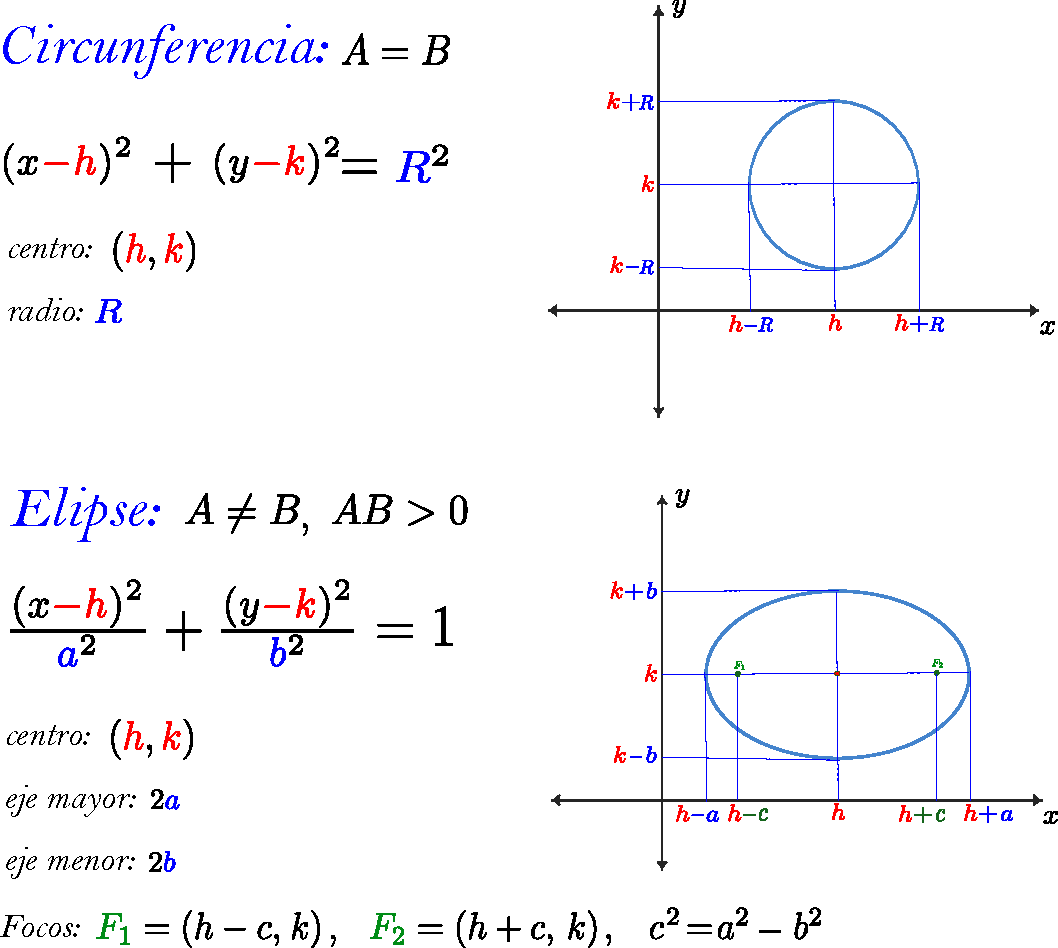
\includegraphics[scale=0.5]{images/elipse.pdf}
    \caption{Esta es una elipse}
    \label{fig01}
\end{figure}

Así se pone la bibliografia:
\bibliographystyle{unsrt}
\bibliography{referecias.bib}

\end{document}